\documentclass[9pt]{beamer}

\useinnertheme{circles}
\useoutertheme{default}
\usecolortheme{orchid}

\setbeamertemplate{navigation symbols}{}

\begin{document}
  
  \title{Algorithms for social networks}
  \subtitle{PageRank}
  \author{Andreea Beica and Baptiste Lefebvre}
  \institute{\'{E}cole Normale Sup\'erieure\\Department of computer science}
  \date{27 january 2014}
  \maketitle

  
\begin{frame}
  \frametitle{Table of contents}
  \tableofcontents
\end{frame}


\section{Introduction}

\begin{frame}
\frametitle{Introduction}
\textbf{PageRank} 
\begin{itemize}
\item assess the importance of a web page based on its relationship with other pages
\item accurate description of user behavior probability
\item objective measure of a web page's importance
\end{itemize}
\end{frame}

\begin{frame}
\frametitle{Introduction}
\begin{figure}[h]
\includegraphics[width=0.8\textwidth]{500px-PageRanks-Example_svg.png}
\caption{Network view of the web}
\end{figure}
\end{frame}

\begin{frame}
\frametitle{Introduction}
\textbf{Text-based search engines:}
\begin{itemize}
\item rely primarily on information contained within the given page
\item titles with a high keyword density, search terms near the beginning of the document
\item easily manipulated, thus unreliable

\end{itemize}

\textbf{Our approach:} PageRank + IR score
\end{frame}



\section{PageRank}


\section{System architecture}


\begin{frame}
\frametitle{System architecture}

\begin{itemize}
\item simulate crawling and indexing the web (difficult)
\item instead: static HTML dumps of all Wikipedia pages for a chosen language
\item all pages are crawled
\item when "crawling" phase is done: graph of hyperlinks + inverted index
\end{itemize}
\end{frame}

\begin{frame}
\frametitle{System architecture}

Steps:

\begin{itemize}
\item Parsing: parse each page, construct \emph{invertedindex} and \emph{pointsTo}
\item Inverted index: used for quick lookup when a query is made
\end{itemize}
\end{frame}

\begin{frame}
\frametitle{System architecture}
\begin{figure}[h]
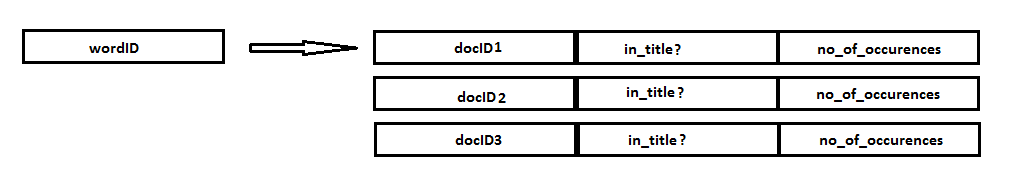
\includegraphics[width=0.8\textwidth]{index.png}
\caption{Simplified inverted index}
\end{figure}
\end{frame}


\begin{frame}
\frametitle{IR score}
Integrated reasoning score:

\begin{itemize}
\item determined by the emphasis and the weighted position of the specific terms in a document
\item used to compute the \emph{actual relevance}  of said document
\item \emph{actual relevance} of a page: IR score * PageRank
\item our (simple) formula: nb$\_$occurences * (in$\_$title+1)
\end{itemize}
\end{frame}

\begin{frame}
\frametitle{Searching}

For simplicity, we only refer to single word queries:
\begin{enumerate}
\item look up query word in inverted index and retrieve corresp. doc list
\item compute IR score for each document
\item combine IR score and PageRank for each document in order to obtain final rank
\item sort documents and return first \emph{k}
\end{enumerate}
\end{frame}






\section{Results}



\section{Conclusions}
\begin{frame}
\frametitle{Conclusions}

\begin{itemize}
\item small functional search engine
\item significant number of pages (15000 in the Afrikaans case)
\item significant size of hyperlink graph
\end{itemize}
\end{frame}

\begin{frame}
\frametitle{Error sources}
\begin{itemize}
\item data fetching
\item outdated databases
\item memory limitations
\item simple models for the inverted index and the IR score
\end{itemize}
\end{frame}

\begin{frame}
  \frametitle{Thanks}
  \begin{center}
    Thanks !
  \end{center}
\end{frame}

\begin{frame}
  \begin{thebibliography}{1}
    \bibitem{brin98}
      S. Brin and L. Page\\
      \begin{bf} The Anatomy of a Large-Scale Hypertextual Web Search Engine \end{bf}\\
      \emph{Computer Networks and ISDN Systems, 1998}
    \bibitem{cho98}
      J. Cho, H. Garcia-Molina, L. Page\\
      \begin{bf} Efficient Crawling Through URL Ordering \end{bf}\\
      \emph{7th International Web Conference, 1998}
  \end{thebibliography}
\end{frame}

\end{document}